\documentclass[12pt]{article}
\usepackage{mathtools}
\usepackage{mdframed}
\usepackage{fullpage}
\usepackage{amsfonts}
\usepackage{tikz}
\usepackage{fancyhdr}
\usepackage{lastpage}
\usepackage{graphicx}
\usepackage{subfig}

\graphicspath{{engl314/instructional/}}


%edit this for each class
\newcommand\name{How to fold a paper plane}
\newcommand\head[1]{\noindent{\large\textbf{#1}}:\newline}

\pagestyle{fancy}
\rfoot{\name, page \thepage/\pageref{LastPage}}
\cfoot{}
\rhead{}
\lhead{}
\renewcommand{\headrulewidth}{0pt}
\renewcommand{\footrulewidth}{0pt}

\title{How to Fold a Paper Airplane}
\author{Group XXDF}

\fontfamily{helvet}

\footnotetext[1]{ Paper airplane is in no way stealthy and will not actually hide your secret messages.
If you throw this plane in a lecture hall or classroom your instructor will see it, and will confiscate it.
No patent exists for paper airplane design. \label{fnt1}}


\begin{document}
\maketitle

\head{Introduction}
\indent Have you ever wanted to send super secret messages across the classroom or lecture hall that no one else was allowed to read? Well, with our patented
stealth paper plane design you can\footnotemark[\ref{fnt1}]! Watch as your stealth plane soars across the skies of your lecture hall.\\

\head{Materials}
\indent One sheet of 8 $\frac{1}{2}''\times 11''$ paper\\
\indent Colored pencils (optional)\\

\head{Instructions}
\begin{figure}[h]
  \centering
  \caption{Fold the paper in half vertically (hotdog style).}
  \subfloat{{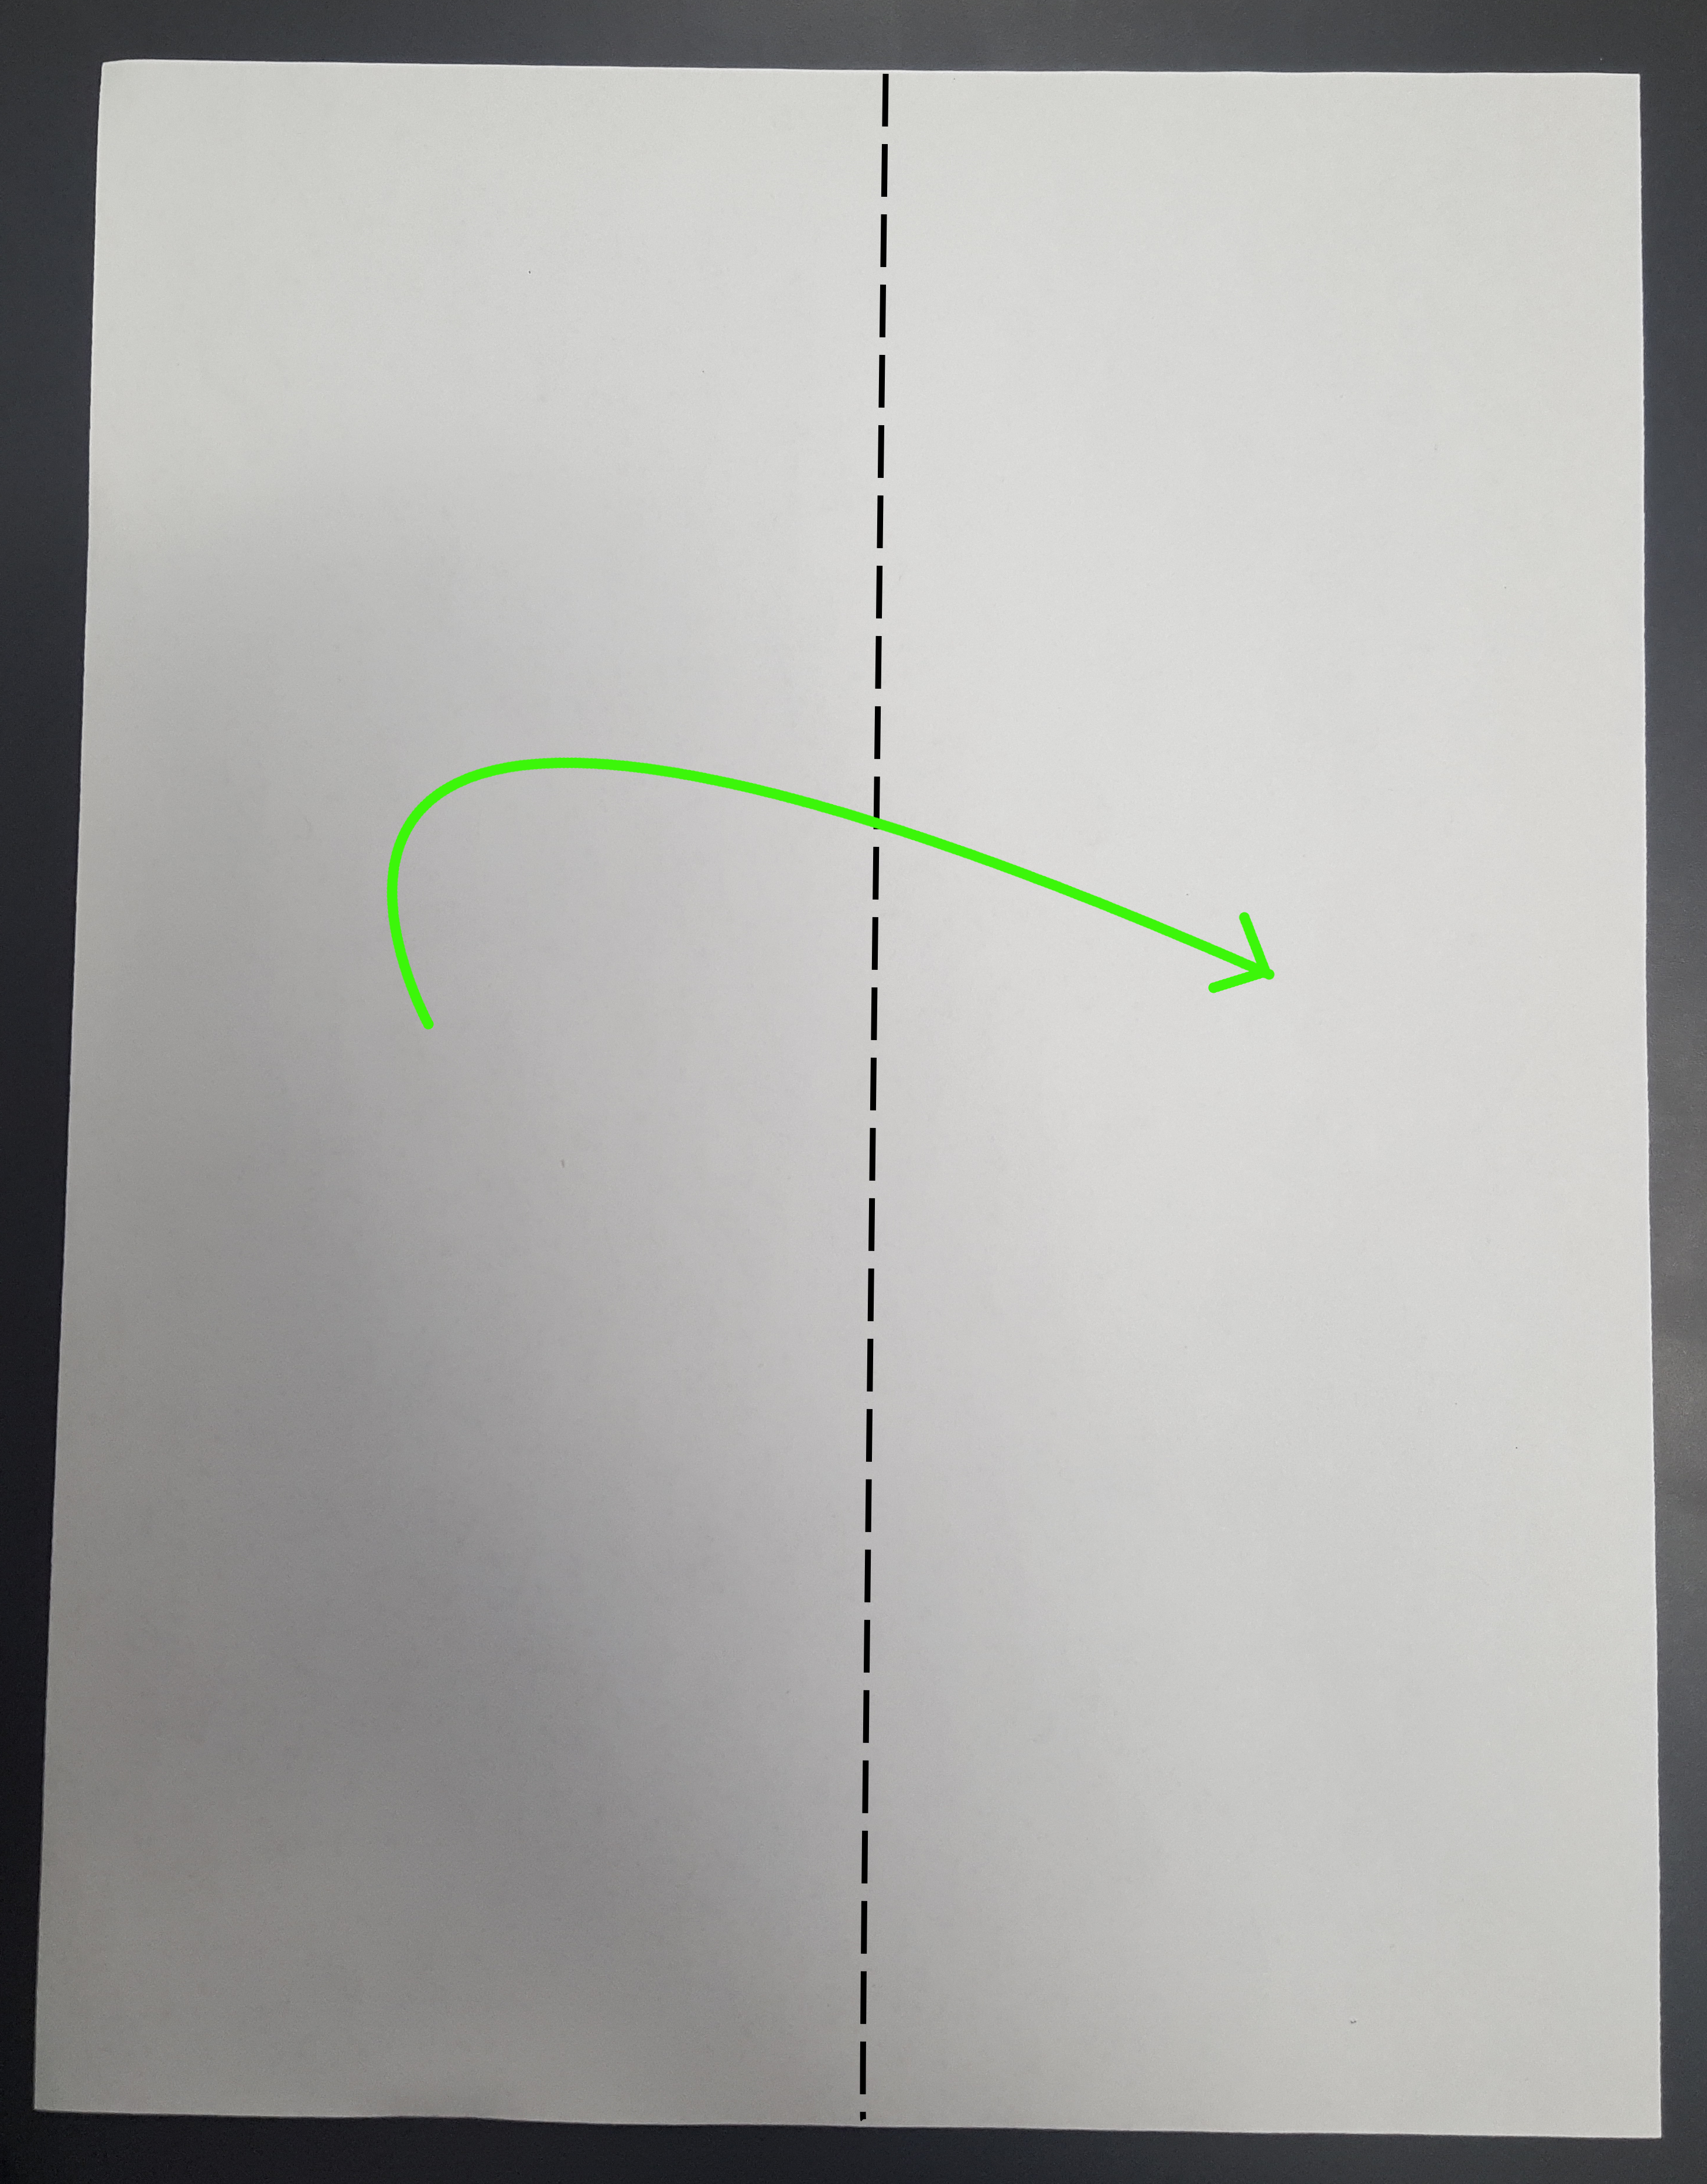
\includegraphics[width=0.33\textwidth]{engl314/instructional/first.png} }}
  \qquad
  \subfloat{{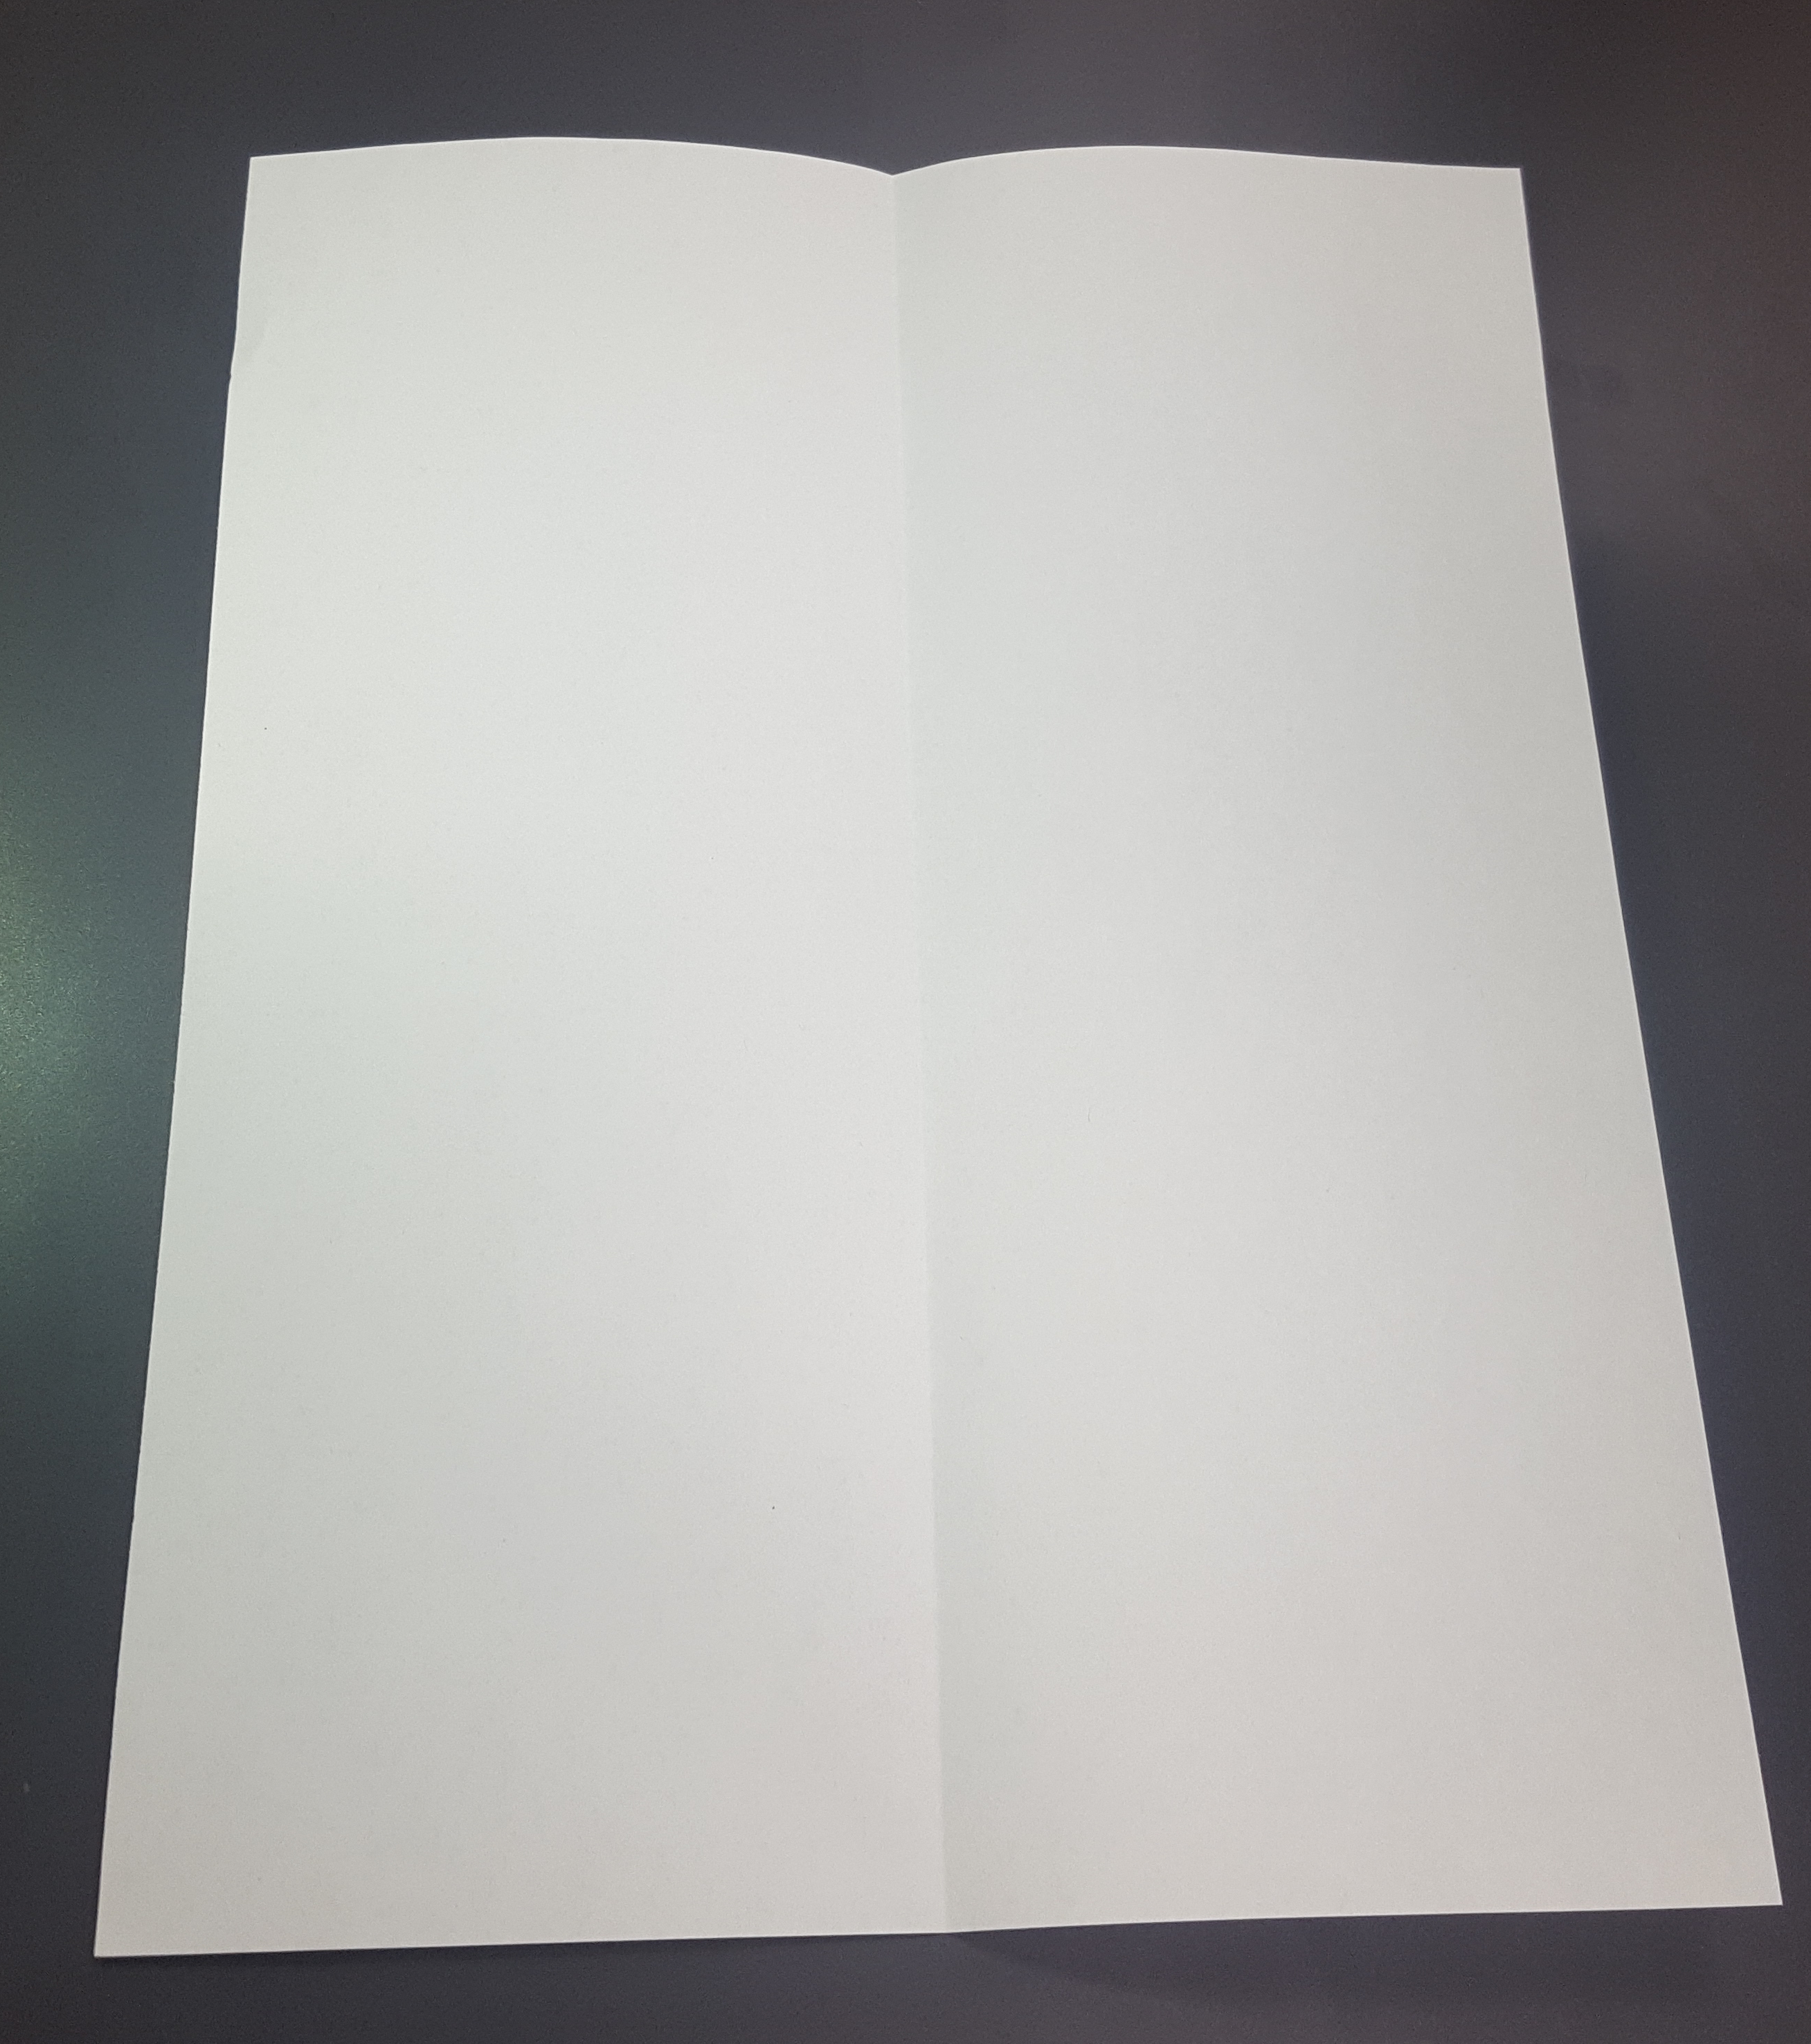
\includegraphics[width=.375\textwidth]{engl314/instructional/second.png} }}
\end{figure}


\end{document}
